\chapter{Climate and Atmosphere Models}
\label{models}
For this study, I used the 3D climate modeling simulations of
 \citet{wolf17,wolf18} as a starting point for analysis of spectral signals that
 may be detected with JWST and other telescopes. Therefore, it is important to
 review the results of the climate models in order to adequately understand any
 conclusions derived from them. Many of the conclusions discussed here will have
 significant impacts on Chapter \ref{spectra} and \ref{tpc}.
 Transit spectra is sensitive to the
 atmospheric composition, and in order to characterize that sensitivity, many
 climate models with varying parameters must be tested. For thermal phase
 curves, clouds are particularly important because they determine the
 emissivity of the atmosphere. Climate models allow us to predict
 the distribution of clouds on the TRAPPIST-1 planets, giving us insight into
 what we would see from a thermal phase curve. Cloud distributions depend on
 the availability of water vapor, the temperature of the planet, and on the
 large scale atmospheric circulation, which itself depends on the strength of
 the Coriolis force, which is determined by the rotational rate of the
 exoplanet. Assuming that the TRAPPIST-1 exoplanets are tidally locked allows us
 to set their rotation rate to their orbital period, allowing us to precisely
 constrain the influence of the Coriolis force.

Climate models have proven to be a very useful tool to accurately predict
 behavior of an atmosphere. Climate models use fundamental physics like
 radiative transfer, convection, the Coriolis force, and other rules to predict
 the motion of air parcels iteratively through time. One popular climate model
 is the Community Atmosphere Model 4 (CAM4), provided by the National Center for
 Atmospheric Research \citep{CAM5}. Using a modified version of CAM4,
 \citet{wolf17, wolf18} were able to apply climate models to the tidally locked
 exoplanets of the TRAPPIST-1 system including TRAPPIST-1 d, TRAPPIST-1 e, and
 TRAPPIST-1 f. All of the climate models for TRAPPIST-1 d entered a runaway
 greenhouse, even in models without \chem{CO_2}. All of the models for
 TRAPPIST-1 f required multi-bar \chem{CO_2} atmospheres to maintain reasonable
 temperatures. TRAPPIST-1 e had numerous models which were habitable with low
 and moderate amounts of \chem{CO_2}, making TRAPPIST-1 e is the most promising
 candidate of the system for supporting habitable conditions. Although other
 cases will be considered, this paper will focus primarily on TRAPPIST-1 e.

Climate models can be used to determine the impacts of a variety of atmospheric
 species. In these models, fixed amounts of \chem{CO_2} and \chem{N_2}
 were given, while \chem{H_{2}O} is allowed to vary self-consistently by CAM4.
 \chem{CO_2} will always tend to warm an atmosphere because of
 the greenhouse effect. Only molecules with 3 or more atoms contribute
 to the greenhouse effect directly because they contain vibrational modes which
 can store energy levels that correspond to infrared wavelengths. Two-atom
 molecules like \chem{N_2} cannot contain vibrational modes, and thus cannot
 absorb or emit infrared light. However, adding \chem{N_2} to an atmospheric
 model will increase the pressure, which can impact the absorption of infrared
 light by \chem{CO_2}. Unlike atomic emission features, which absorb and emit
 at discrete wavelengths, molecular emission features are broad, and although
 they peak at a fixed wavelength, they will emit or absorb light for a large
 range of wavelengths around the peak wavelength. Increasing the pressure of a
 greenhouse gas has the tendency to broaden this emission feature, and therefore
 increase its efficacy as a greenhouse gas. For this reason, adding \chem{N_2}
 to an atmosphere can also increase the atmosphere's average temperature.
 \chem{H_{2}O}, like \chem{CO_2}, is a greenhouse gas and exhibits
 pressure-broadening. More importantly, \chem{H_{2}O} is not well mixed
 in an atmosphere, and may condense in the atmosphere as liquid clouds, ice
 clouds, or vapor, as well as condense on the surface as ice, snow, or water.
 The primary advantage of running a 3D climate model is to allow for
 self-consistent calculations of water in its various phase, as distributed
 across a planet by general circulation.

Recently, Wolf has included \chem{CH_4}, which is a stronger greenhouse gas than
 \chem{CO_2} or
 \chem{H_{2}O}. Shown in Table \ref{modeltable} is a list of all the TRAPPIST-1
 e models used in this study.
 Many of the models for TRAPPIST-1 e have global mean temperatures
 that appear too low or too high to support life. The Earth's mean atmospheric
 temperature is $\sim\SI{287}{\kelvin}$ \citep{meanearthtemp}, and some of the
 models produce similar temperatures. From this list, the most interesting
 models are the $\SI{1}{\bar}$ \chem{N_2}, $\SI{0.2}{\bar}$ \chem{CO_2}, and
 $\SI{1}{\bar}$ \chem{N_2},
 $\SI{0.4}{\bar}$ \chem{CO_2} because they have a global mean temperature
 closest to that of modern day Earth, although some others also stand out as
 strong candidates for habitability.

\begin{table}[htbp]
    \begin{center}
        \begin{tabular}{rrrrr}\hline
            \chem{N_2} & \chem{CO_2} & \chem{CH_4} & \chem{H_2} & Surface Temperature\\
            \si{\bar}& \si{\bar}& \si{\bar}& \si{\bar}& \si{\kelvin} \\ \hline
             0   & 0.25 &  0 &  0   & 237.7\\
             0   & 0.5  &  0 &  0   & 268.0\\
             0   & 1    &  0 &  0   & 303.0\\
             0   & 2    &  0 &  0   & 333.2\\
             0.9 & 0    &  0 &  0.1 & 229.2\\
             1   & 0    &  0 &  0   & 217.4\\
             1   & 0.0004 &  0 &  0   & 234.2\\
             1   & 0.0004 &  $1.7\times10^{-6}$ &  0 & 236.1\\
             1   & 0.01 &  0 &  0   & 248.1\\
             1   & 0.1  &  0 &  0   & 270.2\\
             1   & 0.2  &  0 &  0   & 281.5\\
             1   & 0.4  &  0 &  0   & 301.0\\
             1   & 1    &  0 &  0   & 330.2\\
             1.5 & 0.1  &  0 &  0   & 280.9\\
             1.5 & 0.2  &  0 &  0   & 294.9\\
             2   & 0.1  &  0 &  0   & 286.7\\
             2   & 0.2  &  0 &  0   & 306.1\\
             4   & 0.1  &  0 &  0   & 319.0\\
             4   & 0.2  &  0 &  0   & 332.2\\
             10  & 0.2  &  0 &  0   & 358.4\\ \hline
        \end{tabular}
        \caption[TRAPPIST-1 e Models and Species Abundances]{TRAPPIST-1 e Models
        and Species Abundances. Each row represents a single climate model of
        TRAPPIST-1 e, with each column showing the amount of a given species in
        that model. The surface temperatures are an average of the entire planet
        surface.}
        \label{modeltable}
    \end{center}
\end{table}
Despite what Table \ref{modeltable} and Figure \ref{modelco2plot} suggest,
 habitability is more complicated to define. Most of the details about
 habitability are questions of biology. Many finer details about how life would
 operate cannot be inferred from these models. All of these models use a global
 ocean but ignore ocean currents, which is a major method of heat transport on
 Earth. However, a recent study by \citet{yang19} that used exoplanet GCMs that
 considered ocean currents
 concluded that ocean heat transport is important primarily for cold tidally
 locked planets. Warm tidally locked planets with mean temperatures above 280K
 already have efficient atmospherics heat transport.
 None of the models include land masses, which would change both ocean currents
 and atmospheric currents. Many significant atmospheric species like \chem{O_2},
 \chem{O_3}, \chem{N_2O}, and others are not included, despite their obvious
 significance in Earth's atmosphere. \chem{CO_2} abundance is set as a model
 parameter, but in reality, its abundance would be driven by geologic processes
 over timescales much longer than where CAM4 would be useful. Some geologic
 models of exoplanets have found that negative feedbacks between \chem{CO_2} and
 \chem{H_2O} will tend to cause the partial pressure of \chem{CO_2} to converge
 to a habitable value with liquid water \citep{co2geology}.

In addition to climate models, equations used to predict Earth's atmosphere can
 help us describe the TRAPPIST-1 system. Anthropogenic climate change on Earth
 was predicted by Dr. Svante Arrhenius, who created an effective equation to
 predict the warming of an atmosphere, given an increase in \chem{CO_2}.
 Arrhenius' rule is given as

\begin{equation}
    T=\alpha\ln{\left(\frac{C}{\mathrm{C_0}}\right)}+\mathrm{T_0},
\end{equation}
where $C$ is the current amount of \chem{CO_2} in the atmosphere, $\mathrm{C_0}$
 is the former amount of \chem{CO_2} in the atmosphere at a given time, and
 $\mathrm{T_0}$ is the global atmospheric temperature at that time, $\alpha$ is
 a constant that depends on a number of variables not considered in this model. For
 TRAPPIST-1 e, this equation can be used to interpolate between specific climate
 models. In Figure \ref{modelco2plot},
 this equation produces a reliable line of best fit. A similar fit can be made for
 increasing \chem{N_2}, and is shown in Figure \ref{modeln2plot}.

\begin{figure}[htbp]
    \begin{center}
        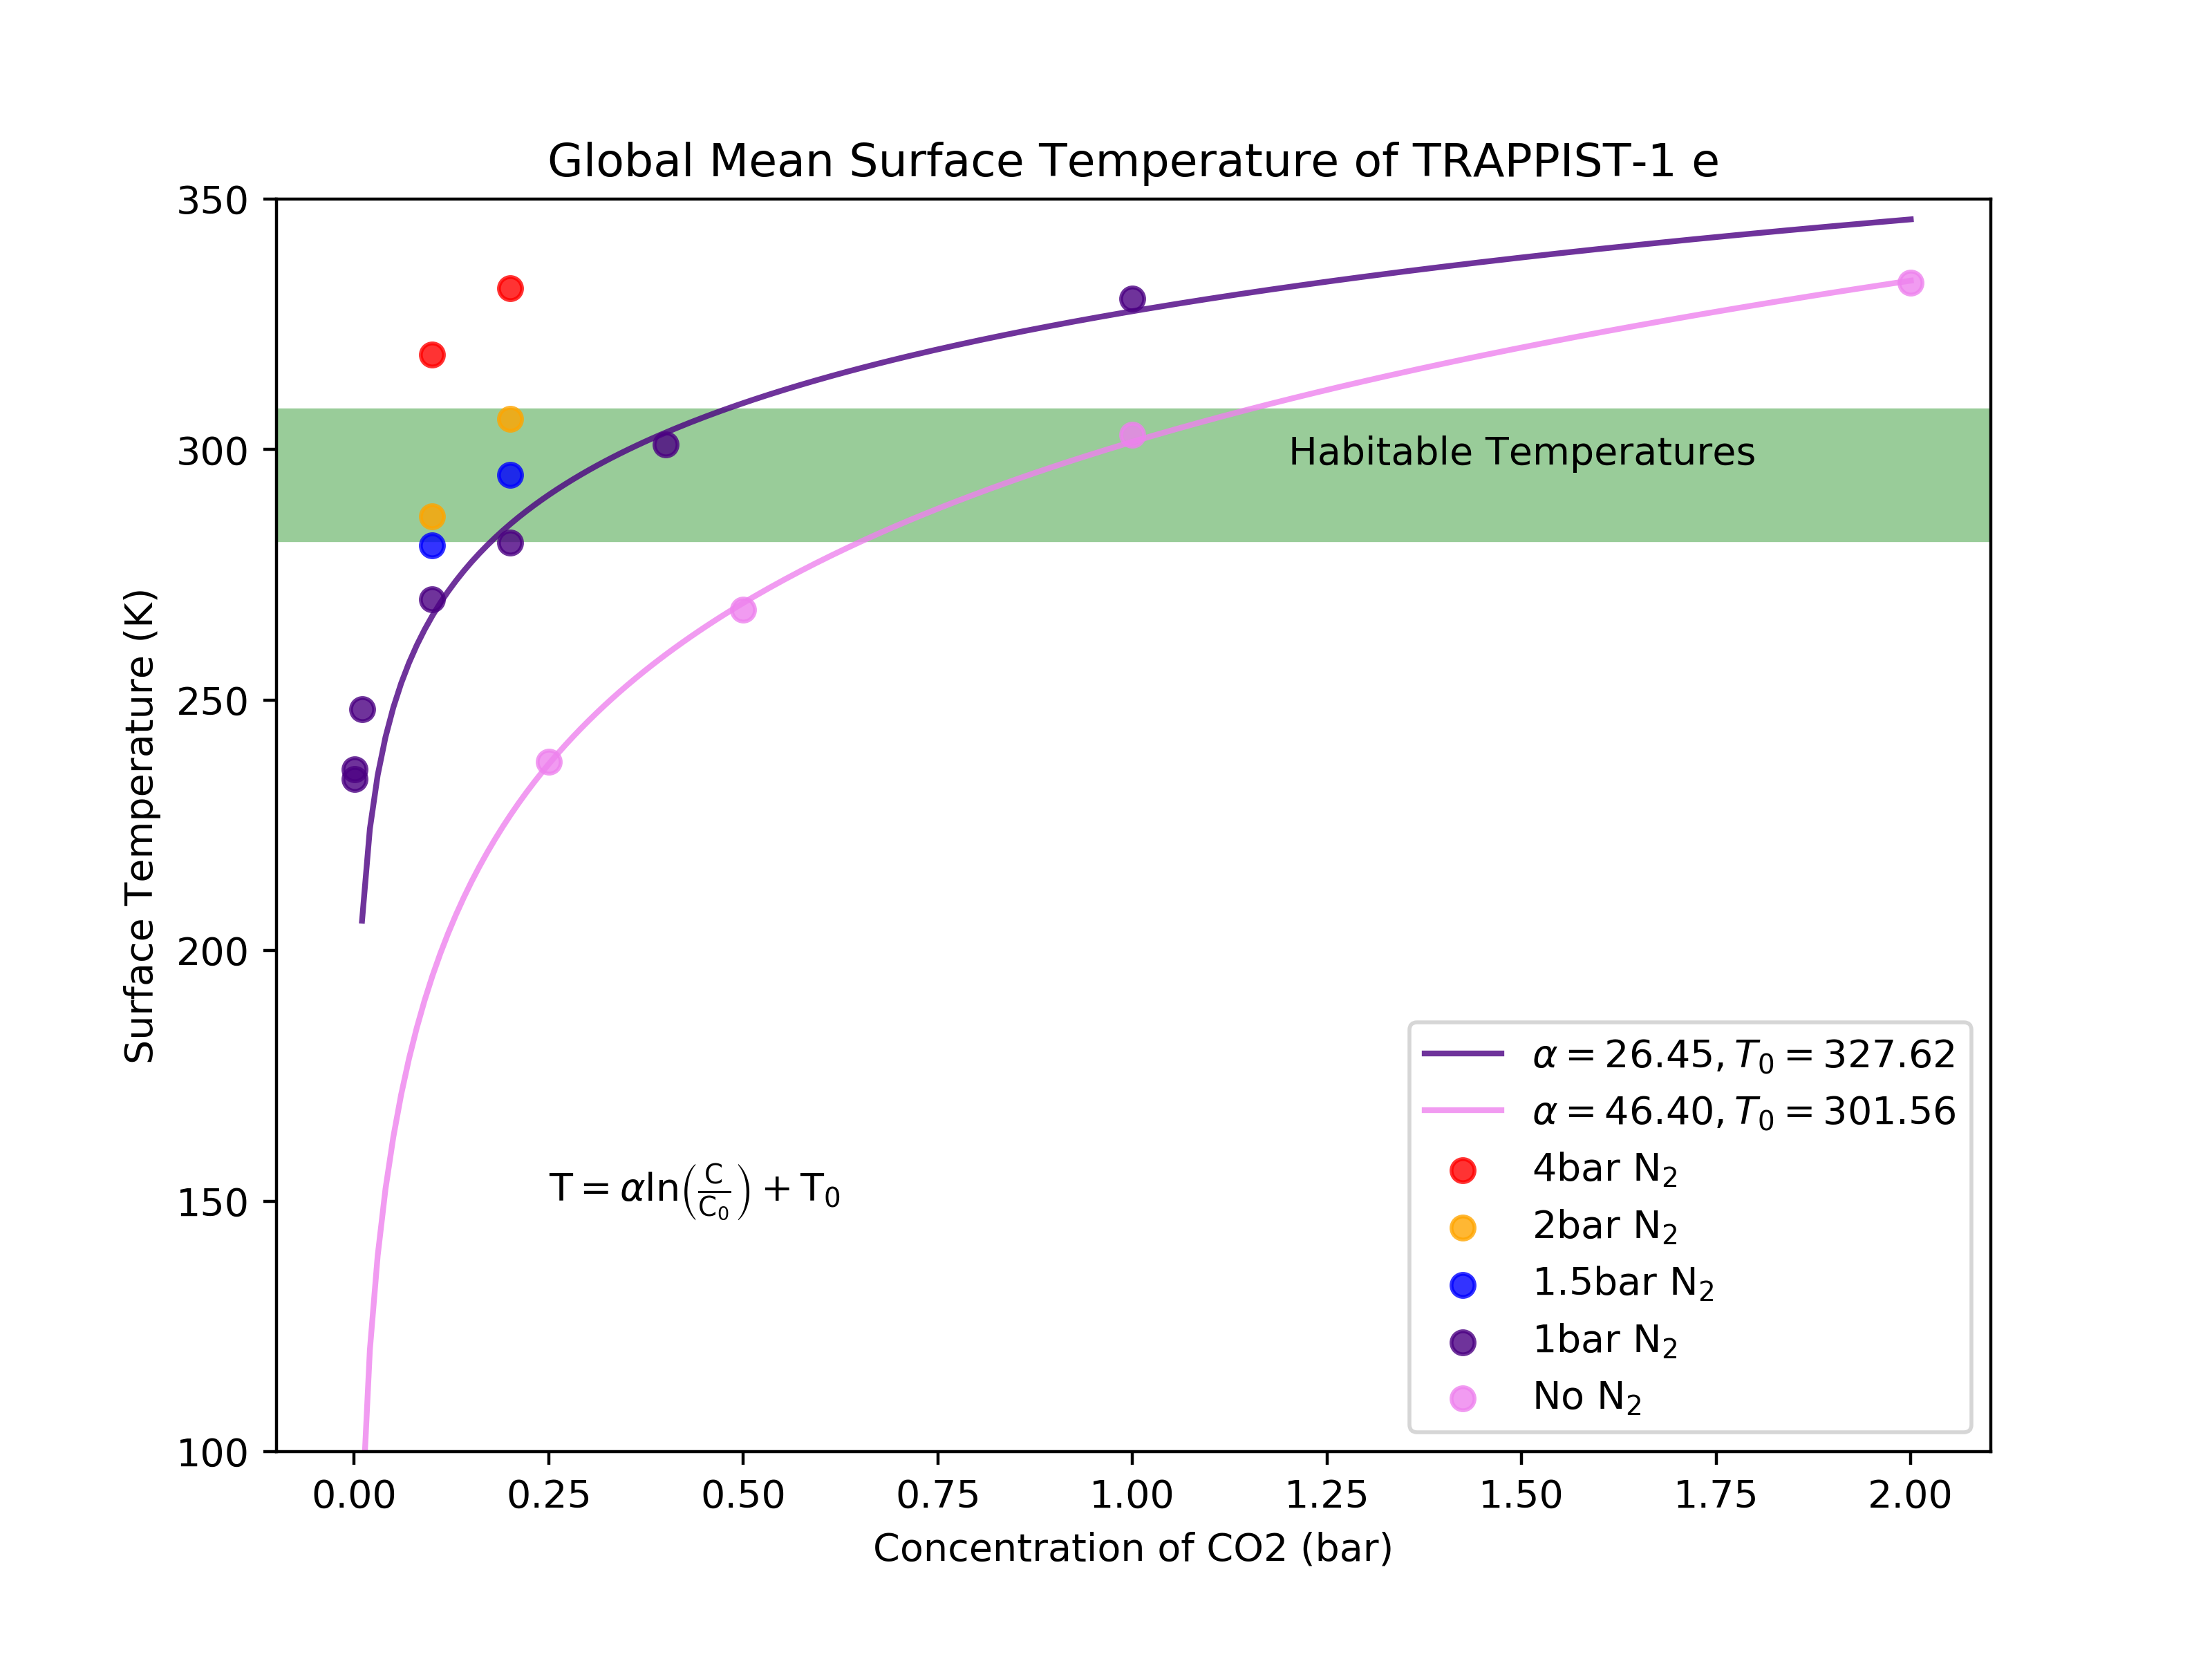
\includegraphics[width=\textwidth]{models/surfacet_co2.png}
        \caption[Globalmean Surface Temperatures Versus \chem{CO_2} Partial
        Pressure]{Globalmean surface temperature versus \chem{CO_2} partial
        pressure. Most of the models in Table \ref{modeltable} are shown here to
        more accurately demonstrate the relationship between \chem{CO_2} and
        warming. Both \chem{CO_2} and \chem{N_2} can contribute significantly to
        the warming of the planet, but they do so differently because \chem{N_2}
        is not a greenhouse gas. In this diagram, the ``habitable zone'' is
        between 275K and 315K, following the definition by \citet{wolf17}.}
        \label{modelco2plot}
    \end{center}
\end{figure}

\begin{figure}[htbp]
    \begin{center}
        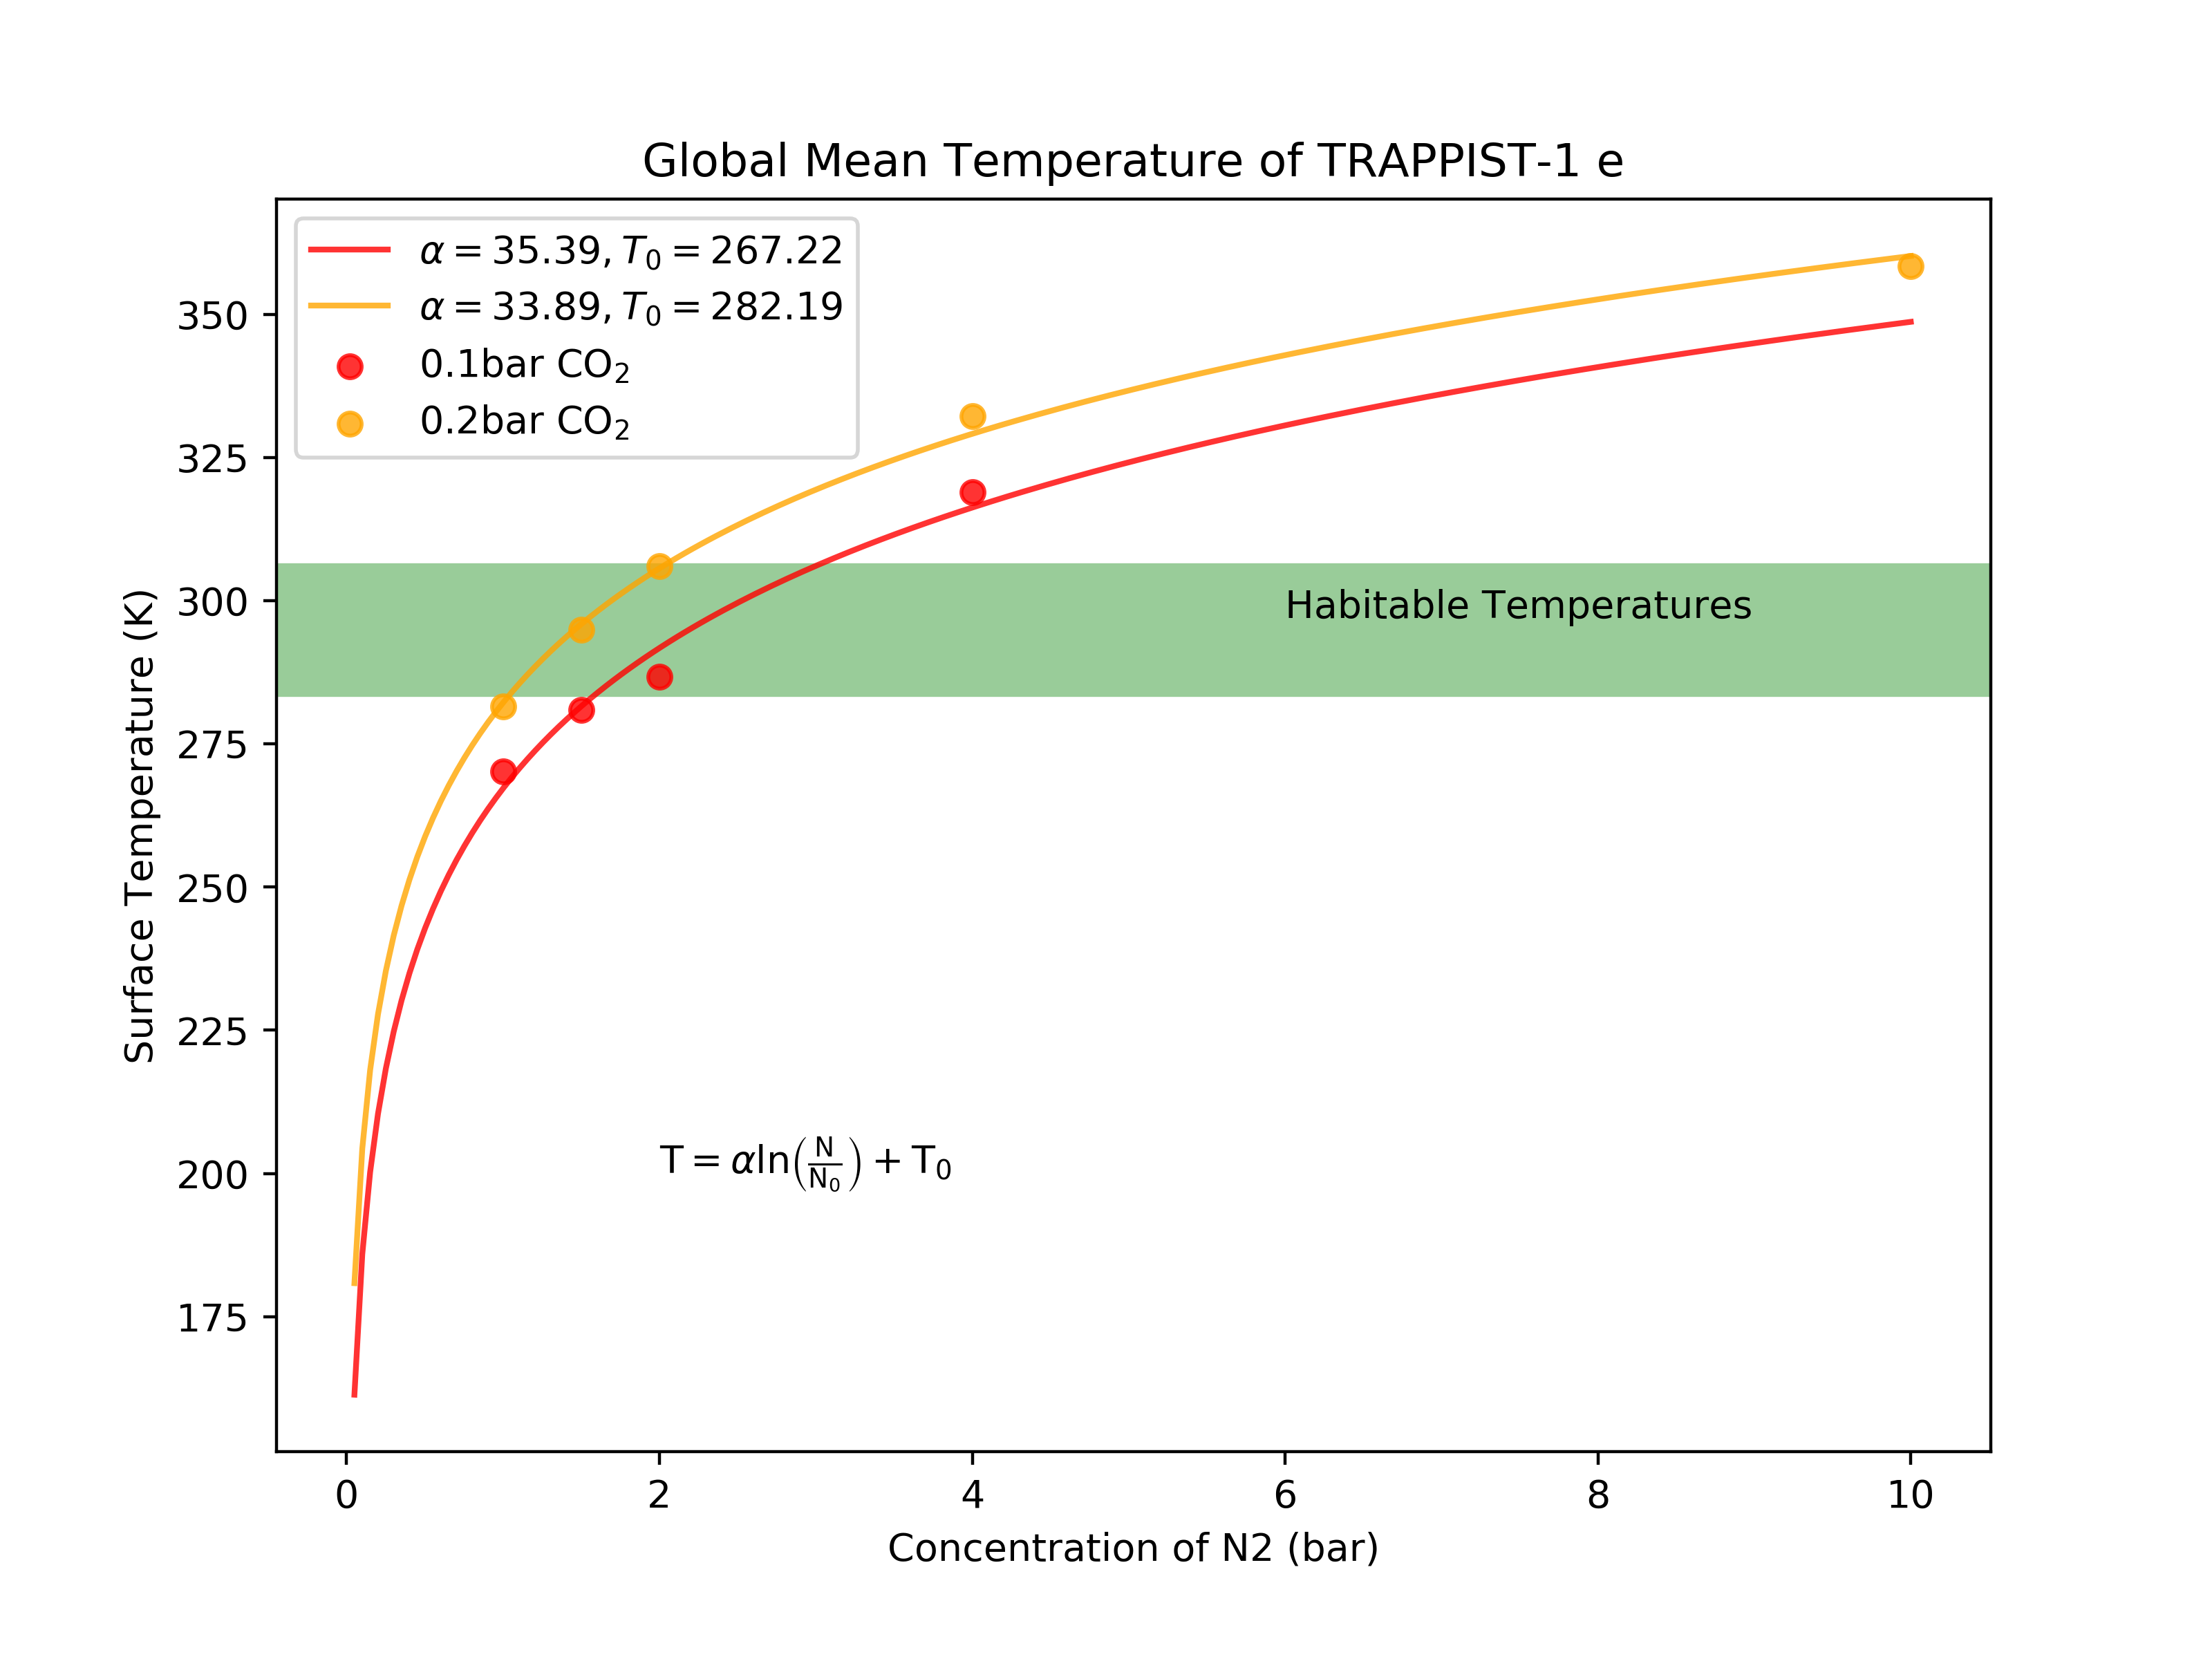
\includegraphics[width=\textwidth]{models/surfacet_n2.png}
        \caption[Globalmean Surface Temperature Versus \chem{N_2} Partial
        Pressure]{Globalmean surface temperature versus \chem{N_2} partial
        pressure. Similarly to Figure \ref{modelco2plot}, logarithmic best fit
        lines match the data well, although the fit is noticably better for
        \chem{CO_2} than \chem{N_2}.}
        \label{modeln2plot}
    \end{center}
\end{figure}

For the purposes of transits, the terminator is the only significant section of
 the atmosphere, but for thermal phase curves, spatial resolution is a
 necessity, largely due to the presence of a substellar cloud
 \citep{ravihabitablemoist}. CAM4 models the atmosphere using a discrete number
 of points, making a 3D array of coordinates where there are 72 longitudinal
 bins, 46 latitudinal bins, and 40 vertical bins. Each attribute of a model
 (like temperature, cloud amount, etc.) all have their own data cubes. In order
 to display the data, it must be reduced from a 3D set. A useful method of
 displaying data like cloud abundance is using a column density. Each vertical
 layer of the atmosphere has a different cloud abundance, but we're mostly
 concerned with \texttt{}he total cloud abundance, which would be the sum of all the
 different layers. This more closely represents what the clouds would look like
 to a distant observer. Figures \ref{clouds} and \ref{precip} are both column
 densities of liquid cloud abundance and precipitation.

A major influence on the structure of clouds in an atmosphere is the Coriolis
 force. The acceleration due to the Coriolis force is given as
 ${\bf a_C}=2 \bf{v}\times{\bf \Omega}$, where {\bf v} is the velocity of a
 particle and $\bf{\Omega}$ is the rotational frequency of the planet. Earth has
 a rotational frequency of $\nicefrac{2\pi}{\SI{24}{\hour}}$, so the Coriolis
 force plays a major role in atmospheric physics. TRAPPIST-1 e has no rotation
 relative to the Sun, but because its year is only 6 days
 \citep{trappistdiscovery}, it will have an angular frequency of
 $\nicefrac{2\pi}{\SI{6}{\day}}$, which is significantly less than Earth's, but
 still strong enough to drive significant zonal circulation. The effects of
 TRAPPIST-1 e's Coriolis force can be clearly seen in Figure \ref{clouds}. The
 substellar cloud is fairly small, and is concentrated to the east, while the
 western side has little to no clouds.

\citet{ravihabitablemoist} has run models on other synchronously rotating
 exoplanets, including some idealized exoplanets with set parameters such as
 solar irradiance and orbital period. These models can be put into two
 categories, fast rotators and slow rotators. An extended orbital period means
 that the Coriolis force is much weaker, which produces a different
 shape for its substellar cloud. The substellar hemisphere is covered by clouds,
 and the substellar cloud is fairly symmetric from the east to west and north to
 south. According to \citet{haqqmisra18}, fast rotators have a period of less
 than 5 days, slow rotators have a period of greater than 20 days, and the
 region in between is called the Rhines rotation regime. TRAPPIST-1 e, on the
 boundary between the two, exhibits characteristics of both. For the purposes of
 this investigation, the most important atmospheric feature is a contained and persistent
 substellar cloud, shown in Figure \ref{clouds}. Slow rotators (like the 44 day
 one shown in Figure \ref{slowrotator} have large substellar clouds that are
 highly symmetric and cover most of the planet's day side.

\begin{figure}[htbp]
    \begin{center}
        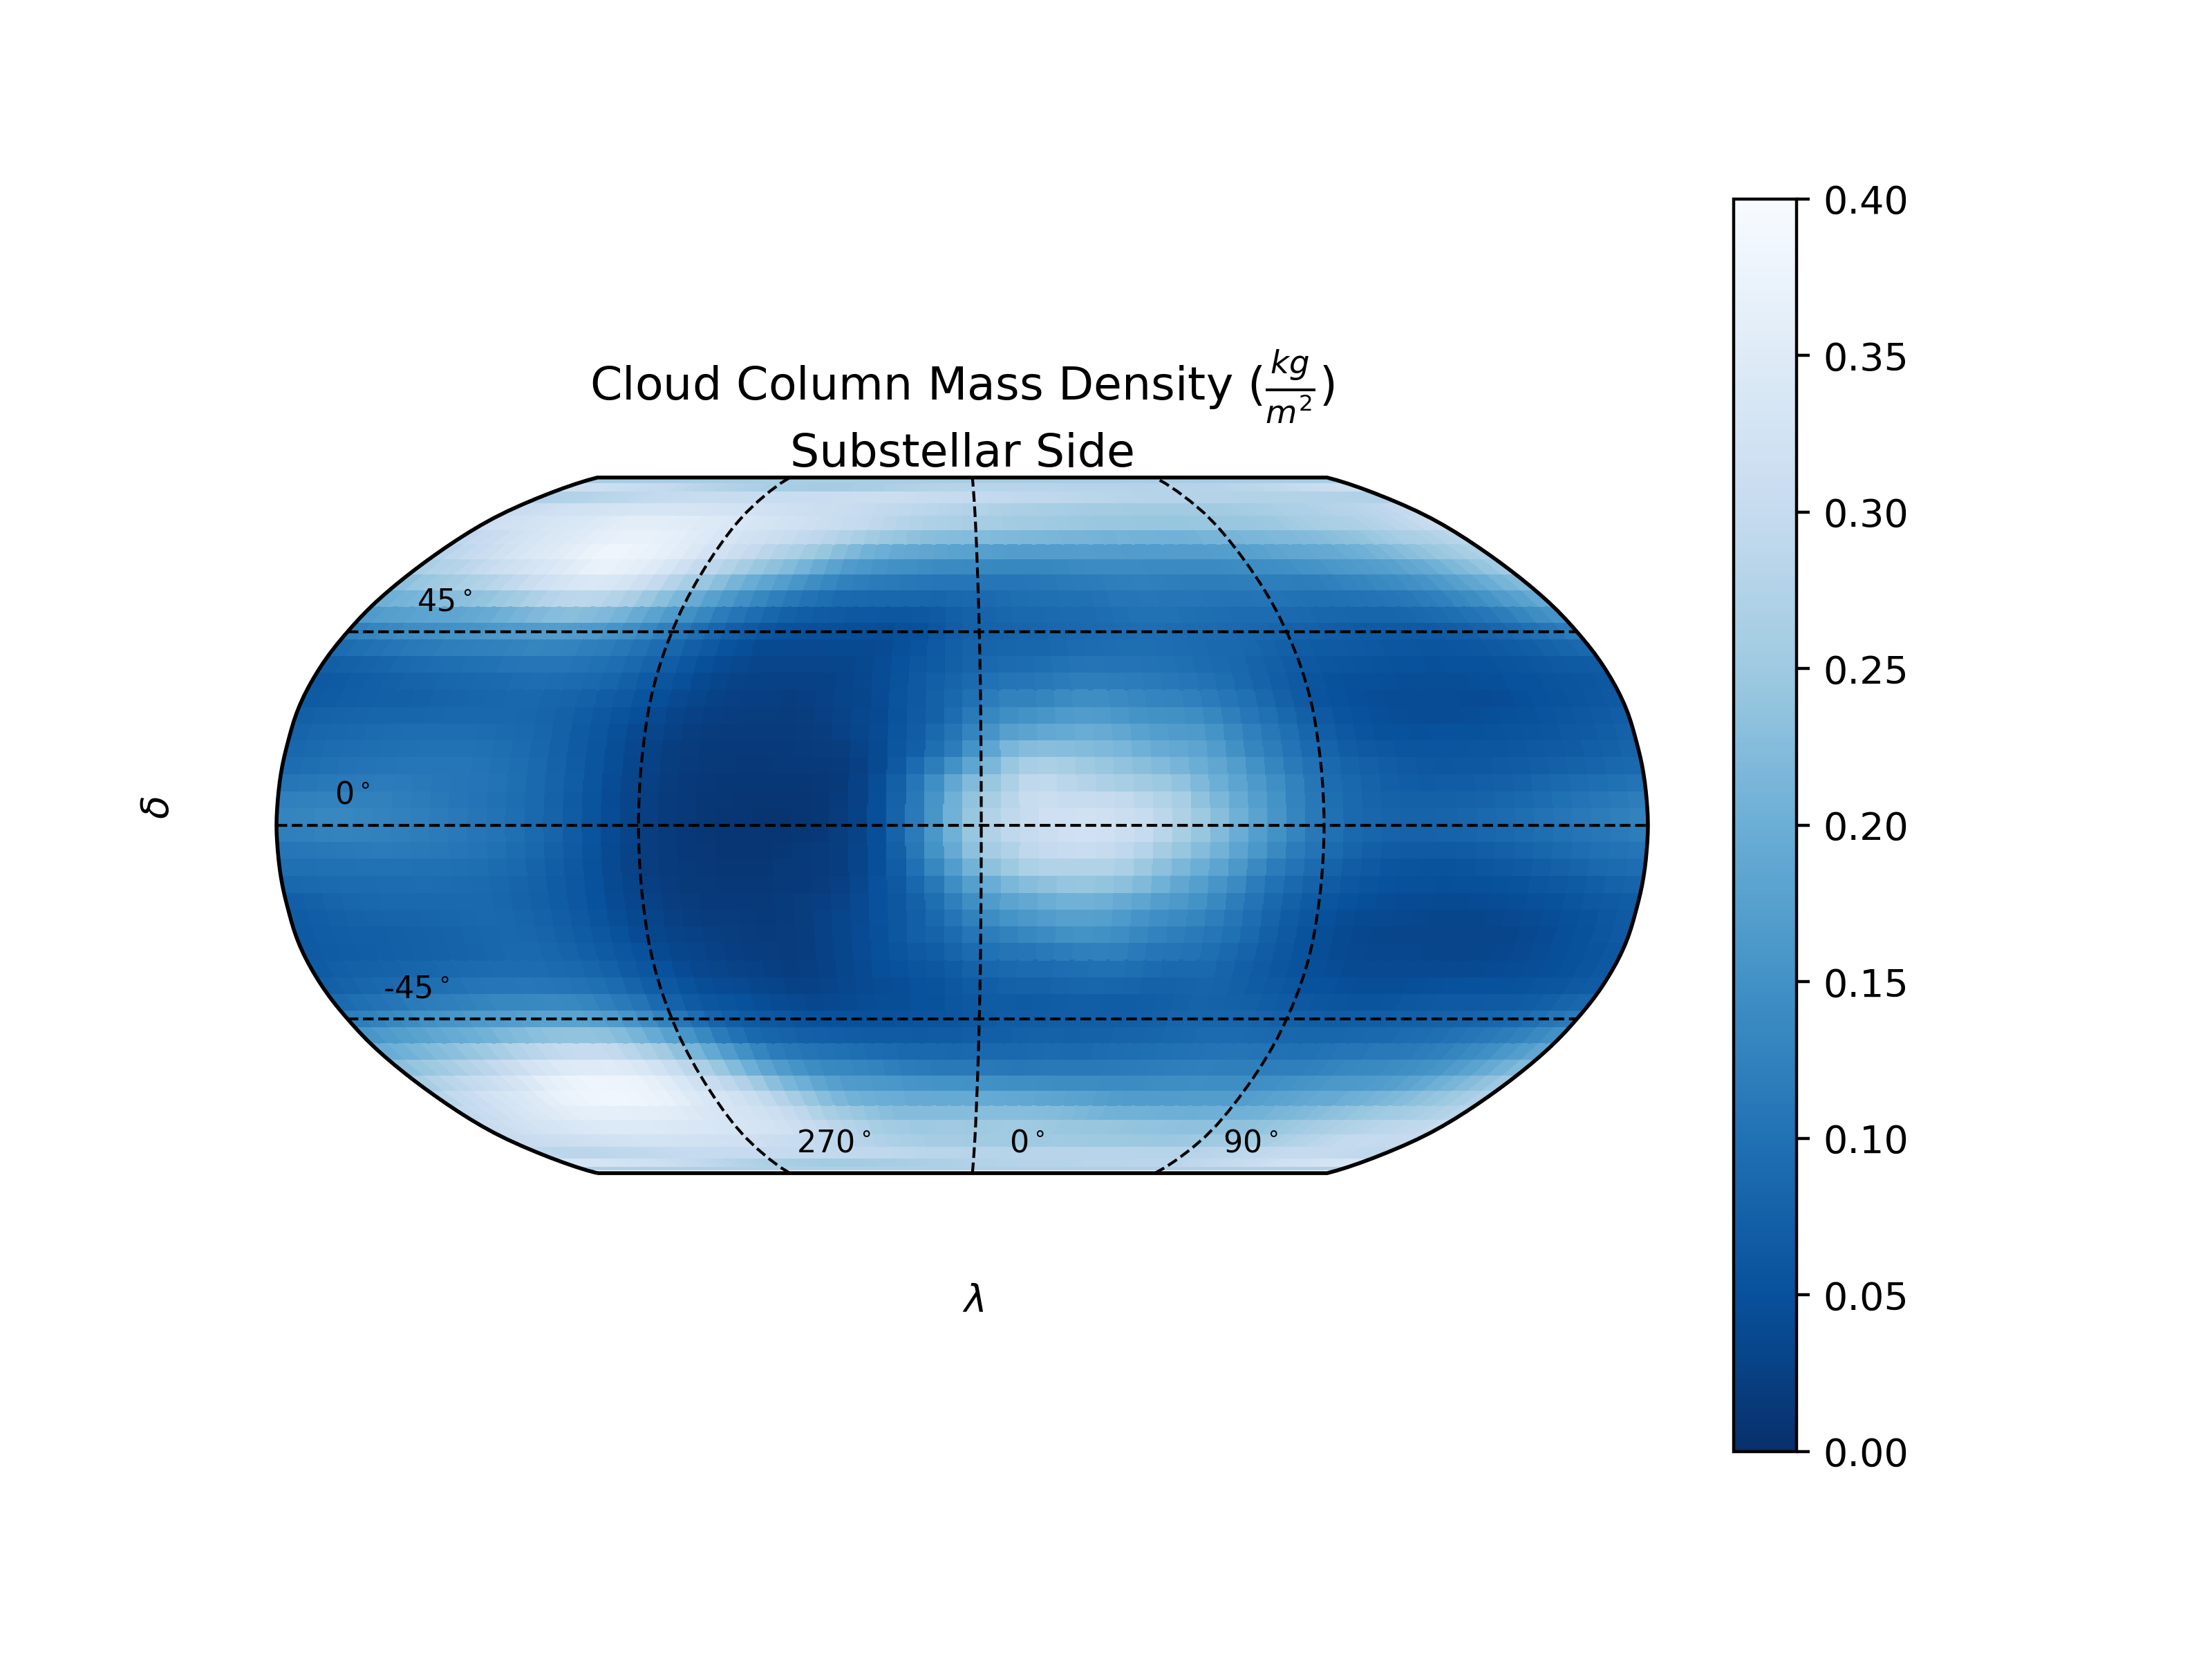
\includegraphics[width=\textwidth]{models/cloud_map.png}
        \caption[Cloud Column Density of TRAPPIST-1 e]{Cloud Column Density of
        TRAPPIST-1 e with $\SI{1}{\bar}$ \chem{N_2} $\SI{0.4}{\bar}$
        \chem{CO_2}. In this image,
        white represents very dense clouds, and blue represents few to no
        clouds. For the substellar point, there are strong clouds, particularly
        on the eastern side. Surprisingly, right next to the substellar point is
        also the region with the least amount of clouds. This is due to the
        planet's rotation, which causes a Coriolis force that produces asymetric
        substellar clouds.}
        \label{clouds}
    \end{center}
\end{figure}

\begin{figure}[htbp]
    \begin{center}
        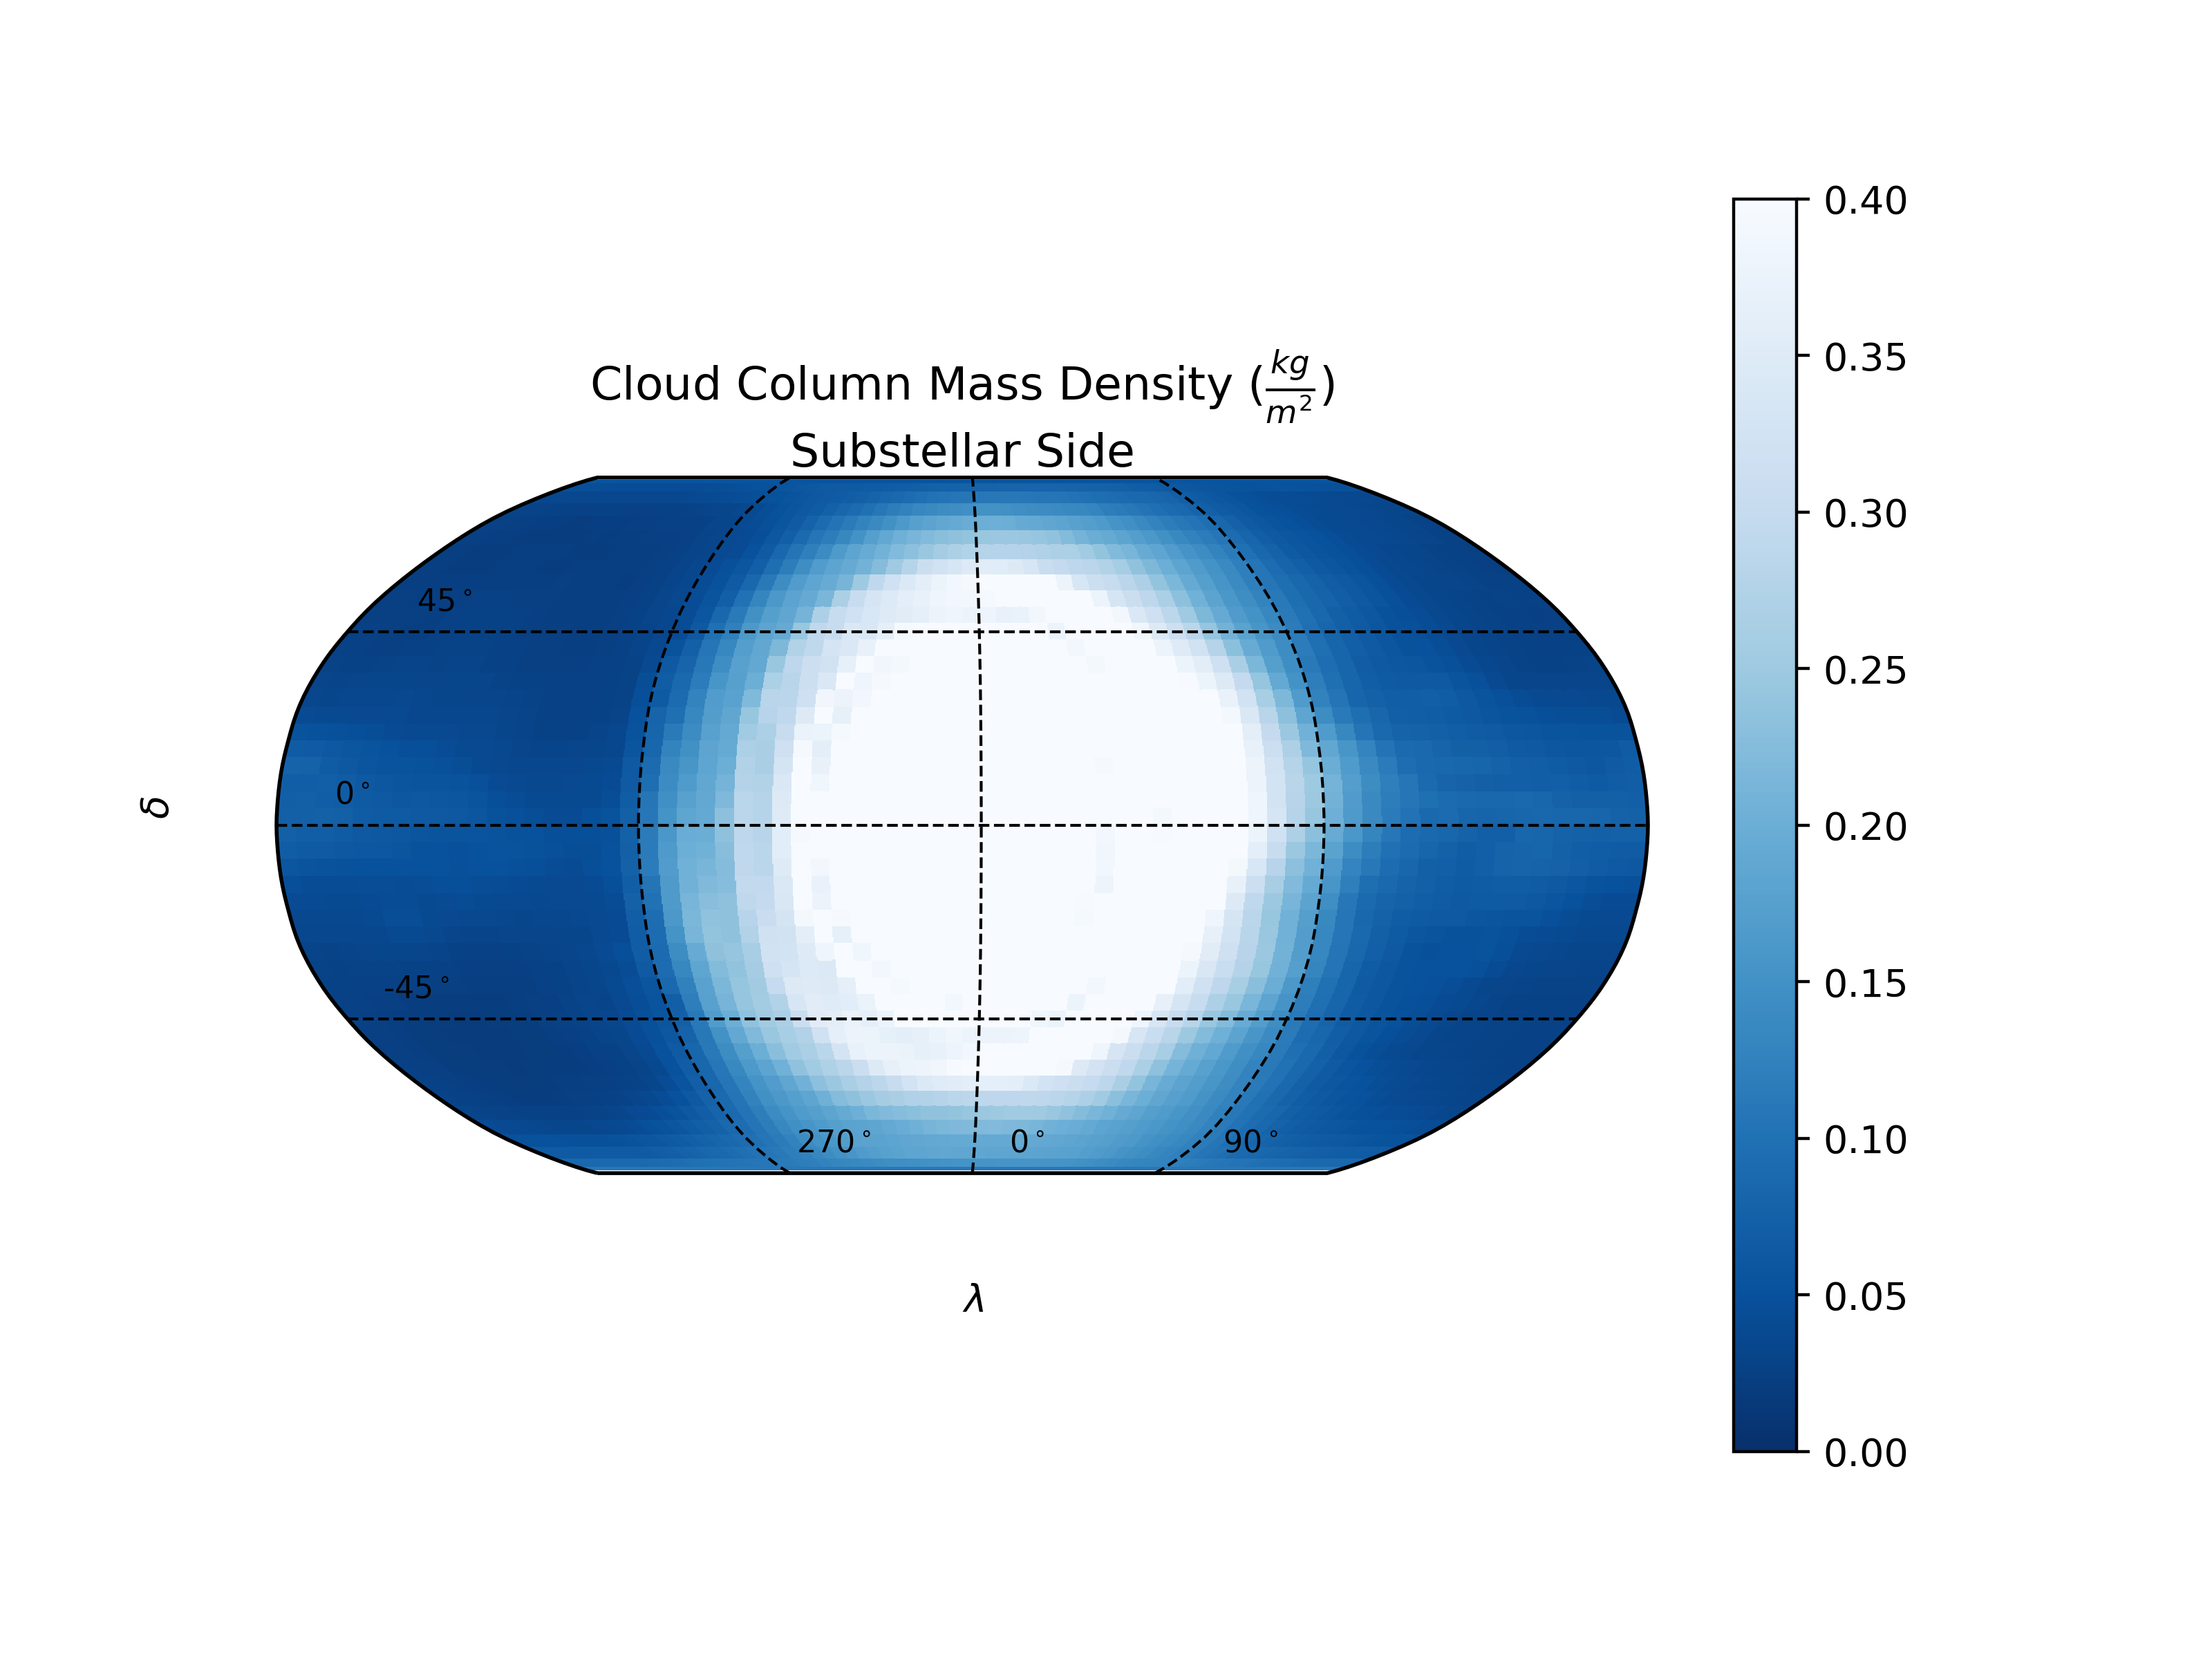
\includegraphics[width=\textwidth]{models/slow_rotator_cloud_map.png}
        \caption[Column Density of a Slow Rotator]{Cloud Column density of a
        slow rotator. The planet used here is a slow rotator with an orbital
        period of 44 days. In this case, it received significantly more solar
        energy from TRAPPIST-1 e, which will cause it to be extremely warm and
        therefore have much stronger clouds than TRAPPIST-1 e. The absolute
        scaling of the cloud amount is less important than the shape of the
        clouds. Here, the clouds are extremely symmetrical and large. This is a
        dramatic difference from the behavior of the TRAPPIST-1 e model in
        Figure \ref{clouds}.}
        \label{slowrotator}
    \end{center}
\end{figure}

\begin{figure}[htbp]
    \begin{center}
        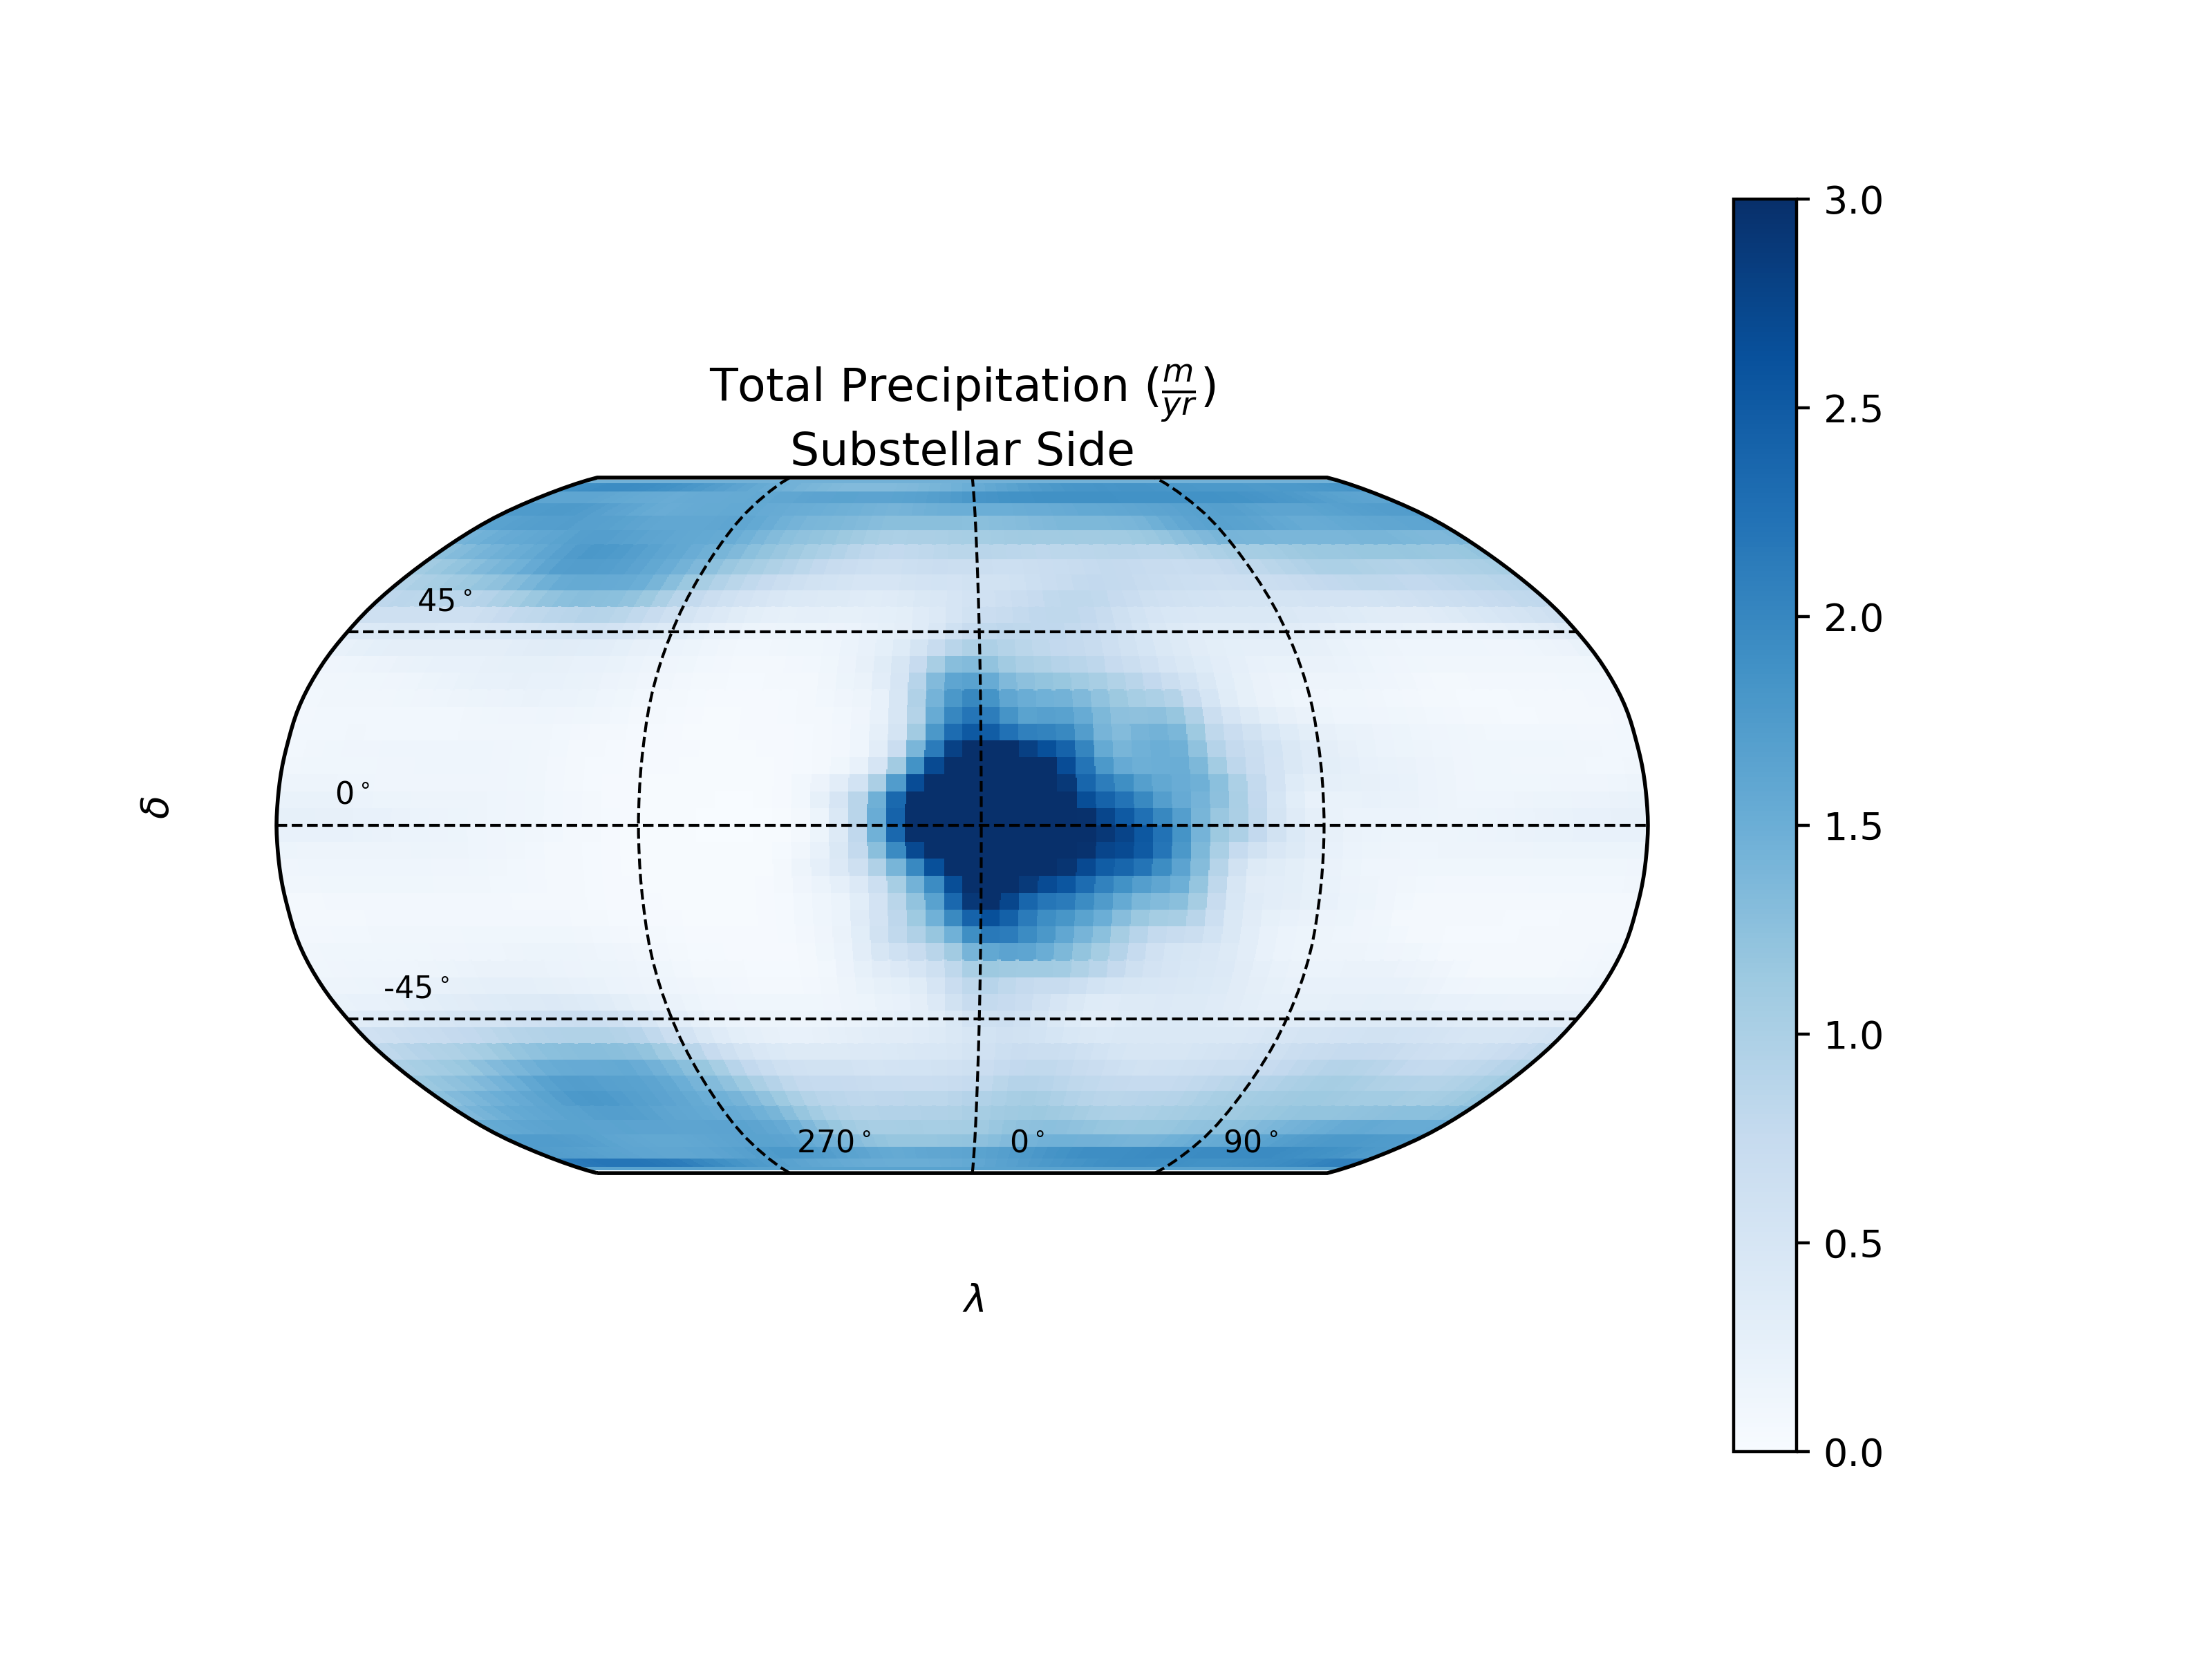
\includegraphics[width=\textwidth]{models/precipitation_map.png}
        \caption[Precipitation of TRAPPIST-1 e]{Precipitation of TRAPPIST-1 e
        with $\SI{1}{\bar}$ \chem{N_2} $\SI{0.4}{\bar}$ \chem{CO_2}. In this
        image, blue represents
        high amounts of precipitation and white represents little to no
        precipitation. From Figure \ref{clouds}, we can conclude there is a
        persistent substellar cloud, but in order to determine if there's
        actually rain reaching the surface, one must also check its
        precipitation since the presence of clouds doesn't always mean there
        must be rain. There does appear to be very localized substellar rain
        indicated by the blue dot, but the rest of the planet only has marginal
        amounts of rain in comparison.}
        \label{precip}
    \end{center}
\end{figure}

In addition to surface features, one of the most useful tools to describe a
 planetary atmosphere is its profile. During an exoplanet transit, light will
 pass through the atmosphere, and the lower atmosphere will be too opaque, and
 little light will make it through, but the upper atmosphere will be much less
 dense, allowing more light through. This means that atmospheric features that
 are close to the planet's surface would be much harder to detect
 compared to upper atmosphere features. Figure \ref{fig:profile} shows that
 a majority of the clouds are concentrated in the lower atmosphere, meaning that
 \chem{H_2O} will be harder to see in an exoplanet transit than \chem{CO_2}
 which is well mixed at all levels of the atmosphere. From Figure
 \ref{fig:profile}, a thermal inversion close to the surface can also be seen,
 meaning that the temperature goes up with height for a brief period. This has
 the effect of stabilizing the atmosphere and on Earth, can cause pollution to
 be trapped near the surface \citep{inversion}. In this plot, the effective
 temperature is given, which is what the temperature of the planet's surface
 would be if it had no atmosphere, and is given by the equation

\begin{equation}
    T_e=\sqrt[4]{\frac{\mathrm{S} (1-\alpha)}{4\mathrm{\sigma}}},
\end{equation}
where $T_e$ is the equilibrium temperature, S is the solar irradiance, $\alpha$
 is the albedo, and $\sigma$ is the Stefan-Boltzmann constant. The equilibrium
 temperature is a useful benchmark for a planetary atmosphere as it represents a
 lower limit on the planet's surface temperature.

\begin{figure}
    \begin{center}
        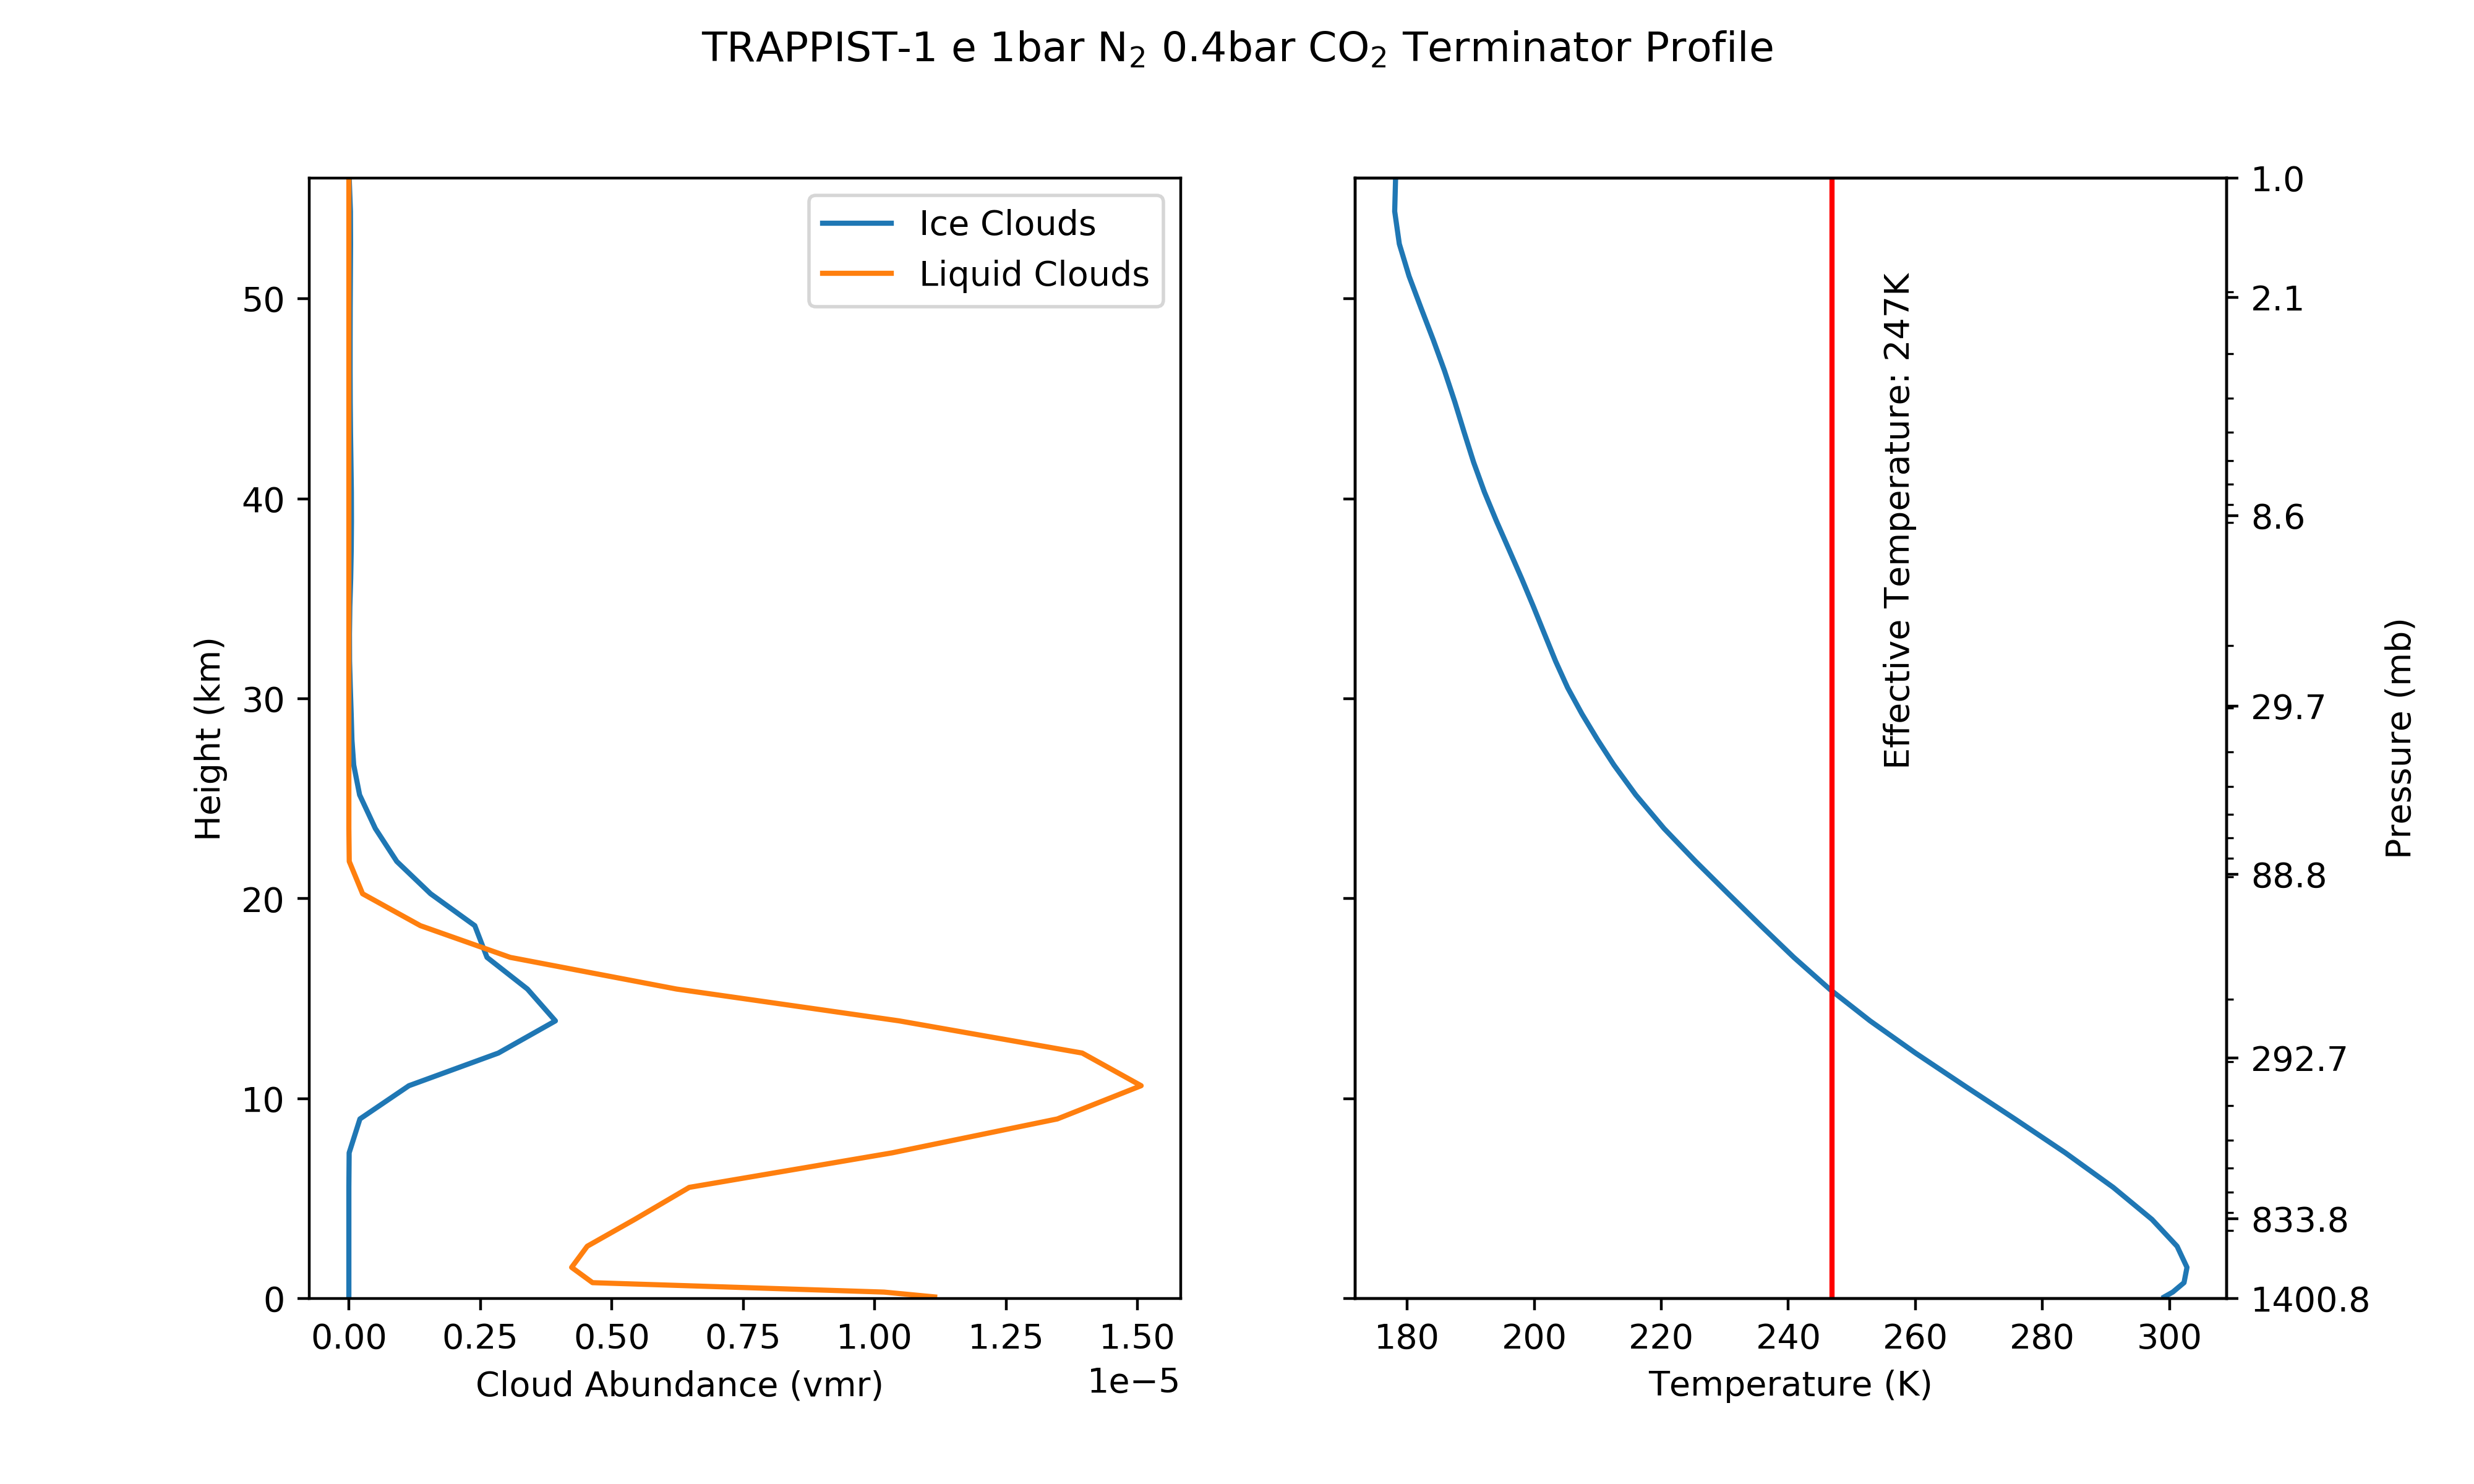
\includegraphics[width=\textwidth]{models/atmosphere_profile.png}
        \caption[TRAPPIST-1 e Atmosphere Profile]{Profile of TRAPPIST-1 e with
        $\SI{1}{\bar}$ \chem{N_2} $\SI{0.4}{\bar}$ \chem{CO_2}. The left plot shows the distribution
        of ice and liquid clouds in the atmosphere. Ice clouds are more abundant
        higher up than liquid clouds. There are also more liquid clouds than
        ice clouds overall, as represented by the surface area under them. The
        right plot is a diagram of temperature across altitude. Close to the
        surface, there is a temperature inversion, stabilizing the surface air.
        Above that, the temperature decreases with height continuously.}
        \label{fig:profile}
    \end{center}
\end{figure}

While these models illustrate many characteristics of the
 TRAPPIST-1 e atmosphere, there are a number of noteworthy assumptions that
 limit our predictive capabilities. These models do not include \chem{O_2}, which
 is a vital element for living organisms. Adding \chem{O_2} would dramatically
 complicate the models because it would require a prognostic chemistry
 calculation, which would imply the addition of \chem{O_3} as well, a greenhouse
 gas and the primary species in the stratosphere. These TRAPPIST-1 e models also do
 not include a stratosphere, which would be a second thermal inversion higher
 up in the atmosphere. These models are long term models run over 40 years, and
 they only have enough resolution to determine general features. Unlike a
 weather forecast model; these models cannot accurately predict small weather
 features in the TRAPPIST-1 e atmosphere, the models are only useful for
 general, long-term trends. These climate models do not include any trace
 atmospheric species, most notably \chem{N_2O}, but there are many more species
 that could be detected during a transit from a telescope.

